% -*- latex -*-
%%%%%%%%%%%%%%%%%%%%%%%%%%%%%%%%%%%%%%%%%%%%%%%%%%%%%%%%%%%%%%%%
%%%%
%%%% This TeX file is part of the course
%%%% Introduction to Scientific Programming in C++/Fortran2003
%%%% copyright 2017-2023 Victor Eijkhout eijkhout@tacc.utexas.edu
%%%%
%%%% loop.tex : loop constructs
%%%%
%%%%%%%%%%%%%%%%%%%%%%%%%%%%%%%%%%%%%%%%%%%%%%%%%%%%%%%%%%%%%%%%

There are many cases where you want to repeat an operation or series
of operations:
\begin{itemize}
\item A time-dependent numerical simulation executes a fixed number of
  steps, or until some stopping test.
\item Recurrences: \[ x_{i+1} = f(x_i). \]
\item Inspect or change every element of a database table.
\end{itemize}


The C++ construct for such repetitions
is known as a~\indextermdef{loop}: a~number of
statements that get repeated. The two types of loop statement in C++ are:
\begin{itemize}
\item the \indextermsub{for}{loop} which is typically associated with
  a pre-determined number of repetitions, and with the repeated
  statements being based on a counter of some sort; and
\item the \indextermsub{while}{loop}, where the statements are
  repeated indefinitely until some condition is satisfied.
\end{itemize}
However, the difference between the two is not clear-cut: in many
cases you can use either.

We will now first consider the \lstinline{for} loop; the \lstinline{while} loop comes in
section~\ref{sec:loopuntil}.

\Level 0 {The `for' loop}
\label{sec:for}

In the most common case, a for loop has a
\indextermbus{loop}{counter}, ranging from some initial value to some 
final value. An example showing the syntax for this simple case is:
\begin{lstlisting}
int sum_of_squares{0};
for (int var=low; var<upper; var++) {
  sum_of_squares += var*var;
}
cout << "The sum of squares from "
     << low << " to " << upper
     << " is " << sum_of_squares << endl;
\end{lstlisting}
The \lstinline{for} line is called the \indextermbus{loop}{header}, and the
statements between curly brackets the \indextermbus{loop}{body}.
Each execution of the loop body is called an
%
\emph{iteration}%
\index{iteration!of a loop|see{loop, iteration}}%
\index{loop!iteration}%
.
\begin{slide}{`For' statement}
  \label{sl:for}
  Sometimes you need to repeat a statement a number of times. That's
  where the \indextermdef{loop} comes in. A~loop has a counter, called
  a~\indexterm{loop variable}, which (usually) ranges from a lower bound
  to an upper bound.

  Here is the syntax in the simplest case:
  \verbatimsnippet{sumsquareloop}
\end{slide}

\begin{exercise}
  \label{ex:manyhello}
  Read an integer value with \lstinline{cin}, and print `Hello world' that many times.
\end{exercise}
\begin{exercise}
  \label{ex:counthello}
  Extend exercise~\ref{ex:manyhello}: the input 17 should now give lines
\begin{verbatim}
Hello world 1
Hello world 2
....
Hello world 17
\end{verbatim}
Can you do this both with the loop index starting at 0 and~1?\\
Also, let the numbers count down.
\end{exercise}

We will now investigate the components of a loop.

\Level 1 {Loop variable}

First of all, most \lstinline{for} loops have a
\indextermbus{loop}{variable} or \indextermbus{loop}{index}.
The first expression in the parentheses
is usually concerned with the initialization of this variable:
it is executed once, before the loop iterations.
If you declare a variable here, it becomes local to the loop,
that is, it only exists in the expressions of the loop header,
and during the loop iterations.

\begin{block}{Loop syntax: variable}
  \label{sl:for-syntax1}
  The loop variable is usually an integer:
\begin{lstlisting}
for ( int index=0; index<max_index; index=index+1) {
  ...
}
\end{lstlisting}
  But other types are allowed too:
\begin{lstlisting}
for ( float x=0.0; x<10.0; x+=delta ) {
  ...
}
\end{lstlisting}
Beware the stopping test for non-integral variables!
\end{block}

Usually, the loop variable only has
meaning inside the loop so it should only be defined there.
You do this by defining it  in the loop header:
\begin{lstlisting}
for (int var=low; var<upper; var++) {
\end{lstlisting}

However, it can also be defined outside the loop:
\begin{lstlisting}
int var;
for (var=low; var<upper; var++) {
\end{lstlisting}
but you should only do this if the variable
is actually needed after the loop.
You will see an example where this makes sense
below in section~\ref{sec:loopuntil}.
 
\Level 1 {Stopping test}

Next there is a test,
which needs to evaluate to a boolean expression.
This test is often called a `stopping test',
but to be technically correct it is actually executed
at the start of each iteration, including the first one,
and it is really a `loop while this is true' test.
%
\snippetwithoutput{pretest}{basic}{pretest}

\begin{block}{Loop syntax: test}
  \label{sl:for-syntax2}
  \begin{itemize}
  \item If this boolean expression is true, do the next iteration.
  \item Done before the first iteration too!
  \item Test can be empty. This means no test is applied.
  \end{itemize}
\begin{lstlisting}
for ( int i=0; i<N; i++) {...}
for ( int i=0; ; i++ ) {...}
\end{lstlisting}
\end{block}

Usually, the combination of the initialization and the stopping test
determines how many iterations are executed.
If you want to perform $N$ iterations you can write
\begin{lstlisting}
for (int iter=0; iter<N; iter++)
\end{lstlisting}
or
\begin{lstlisting}
for (int iter=1; iter<=N; iter++)
\end{lstlisting}
The former is slightly more idiomatic to~C++,
but you should write whatever best fits the problem you are coding.

The stopping test doesn't need to be an upper bound. Here is an
  example of a loop that counts down to a lower bound.
\begin{lstlisting}
for (int var=high; var>=low; var--) { ... }
\end{lstlisting}

The stopping test can be omitted
\begin{lstlisting}
for (int var=low; ; var++) { ... }
\end{lstlisting}
if the loops ends in some other way. You'll see this later.

\Level 1 {Increment}

Finally, after each iteration we need to update the loop variable.
Since this is typically adding one to the variable we can
informally refer to this as the `increment', but
it can be a more general update.

\begin{block}{Loop syntax: increment}
  \label{sl:for-syntax3}
  %%more-increment
  Increment performed after each iteration. Most common:
  \begin{itemize}
  \item \lstinline{i++} for a loop that counts forward;
  \item \lstinline{i--} for a loop that counts backward;
  \end{itemize}
  Others:
  \begin{itemize}
  \item \lstinline{i+=2} to cover only odd or even numbers, depending on
    where you started;
  \item \lstinline{i*=10} to cover powers of ten.
  \end{itemize}
  Even optional:
\begin{lstlisting}
for (int i=0; i<N; ) {
  // stuff
  if ( something ) i+=1; else i+=2; 
}
\end{lstlisting}
\end{block}

This is how a loop is executed.
\begin{itemize}
\item The initialization is performed.
\item At the start of each iteration, including the very first, the
  stopping test is performed. If the test is true, the iteration is
  performed with the current value of the loop variable(s).
\item At the end of each iteration, the increment is performed.
\end{itemize}

\begin{cnote}
  Declaring the loop variable in the loop header is also a modern
  addition to the C~language.
  Use compiler flag \n{-std=c99}.
\end{cnote}


\begin{exercise}
  \label{ex:sumevensquares}
  Take this code:
  \verbatimsnippet{sumsquareloop}
  and modify it to sum
  only the squares of every other number, starting at \lstinline{low}.

  Can you find a way to sum the squares of the even numbers $\geq$\lstinline{low}?
\end{exercise}

\begin{review}
  \label{q:loop1}
  For each of the following loop headers, how many times is the body
  executed? (You can assume that the body does not change the loop variable.)

\begin{lstlisting}
for (int i=0; i<7; i++)
\end{lstlisting}
\slackpoll{"\n{for (int i=0; i<7; i++)}" "6 iterations" "7" "8"}

\begin{lstlisting}
for (int i=0; i<=7; i++)
\end{lstlisting}
\slackpoll{"\n{for (int i=0; i<=7; i++)}" "6 iterations" "7" "8"}

\begin{lstlisting}
for (int i=0; i<0; i++)
\end{lstlisting}
\slackpoll{"\n{for (int i=0; i<0; i++)}" "0 iterations" "1" "inf"}
\end{review}


\begin{review}
  \label{q:loop2}
  What is the last iteration executed?
  \begin{lstlisting}
    for (int i=1; i<=2; i=i+2)
  \end{lstlisting}
  \slackpoll{"\n{for (int i=1; i<=2; i=i+2)} last iteration" "i=1" "i=2" "i=3" "i=4"}

  \begin{lstlisting}
    for (int i=1; i<=5; i*=2)
  \end{lstlisting}
  \slackpoll{"\n{for (int i=1; i<=5; i*=2)} last iteration" "4" "5" "8"}

  \begin{lstlisting}
    for (int i=0; i<0; i--)
  \end{lstlisting}
  \slackpoll{"\n{for (int i=0; i<0; i--)} last iteration" "none" "0" "-1" "-inf"}

  \begin{lstlisting}
    for (int i=5; i>=0; i--)
  \end{lstlisting}
  \slackpoll{"\n{for (int i=5; i>=0; i--)} last iteration" "0" "1" "-1" "4"}

  \begin{lstlisting}
    for (int i=5; i>0; i--)
  \end{lstlisting}
  \slackpoll{"\n{for (int i=5; i>0; i--)} last iteration" "0" "1" "-1" "4"}
\end{review}


\Level 1 {Loop body}

The loop body can be a single statement:
\begin{lstlisting}
int s{0};
for ( int i=0; i<N; i++)
  s += i;
\end{lstlisting}
or a block:
\begin{lstlisting}
int s{0};
for ( int i=0; i<N; i++) {
  int t = i*i;
  s += t;
}
\end{lstlisting}
If it is a block, it is a scope inside which you can declare local variables.

\Level 0 {Nested loops}

Quite often, the loop body will contain another loop. For instance,
you may want to iterate over all elements in a matrix. Both loops will
have their own unique loop variable.
\begin{lstlisting}
for (int row=0; row<m; row++)
  for (int col=0; col<n; col++)
    ...
\end{lstlisting}
This is called \indextermbus{loop}{nest}; 
the \lstinline{row} loop is called the \indextermsub{outer}{loop} and the
\lstinline{col} loop the \indextermsub{inner}{loop}.

\begin{slide}{Nested loops}
  \label{sl:for-nest}
  Traversing a matrix\\
  (we will discuss actual matrix data structures later):
\begin{lstlisting}
for (int row=0; row<m; row++)
  for (int col=0; col<n; col++)
    ...
\end{lstlisting}
This is called `loop nest', with\\
\lstinline{row}: outer loop\\
\lstinline{col}: inner loop.
\end{slide}

Traversing an index space (whether that corresponds to an array object
or not) by \lstinline{row,col} is called the \indexterm{lexicographic ordering}.

\begin{exercise}
  \label{ex:ij-triangle}
  Write an $i,j$ loop nest that prints out all pairs with
  \[ 1\leq i,j\leq 10,\quad  j\leq i. \]
  Output one line for each \lstinline{i} value.

  Now write an $i,j$ loop that prints all pairs with
  \[ 1\leq i,j\leq 10,\quad |i-j|<2, \]
  again printing one line per \lstinline{i} value.
  Food for thought: this exercise is definitely easiest with a
  conditional in the inner loop, but can you do
  it without? 
\end{exercise}

\begin{figure}[ht]
  \hbox{%
    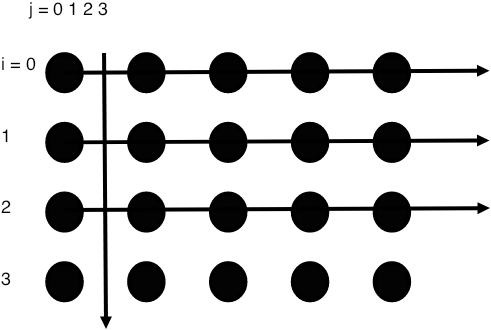
\includegraphics[scale=.4]{ij-lexicographic}
    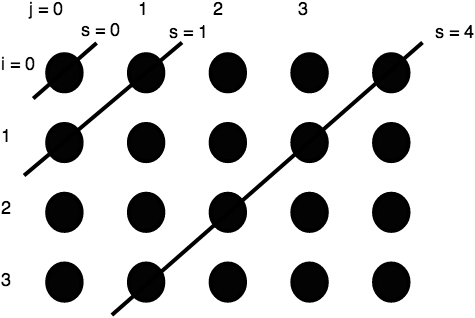
\includegraphics[scale=.4]{ij-by-diagonal}
    }
  \caption{Lexicographic and diagonal ordering of an index set}  
  \label{fig:ij-lex}
\end{figure}

The mere fact that you need to traverse a rectangular range
of $i,j$ indices,
does not mean that you have to write a lexicographically
indexed loop.
Figure~\ref{fig:ij-lex} illustrates that you can look at the $i,j$
indices by row/column or by diagonal. Just like rows and columns being
defined as $i=\mathrm{constant}$ and $j=\mathrm{constant}$
respectively,
a diagonal is defined by $i+j=\mathrm{constant}$.

\begin{figure}[ht]
  \hbox{%
    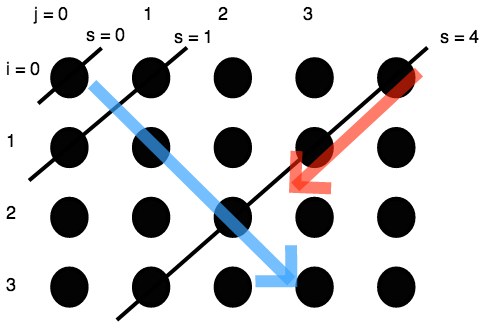
\includegraphics[scale=.4]{ij-by-diagonal-arrow}
    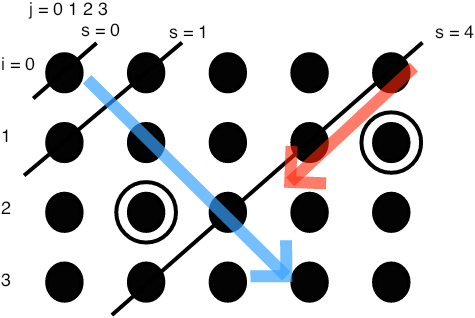
\includegraphics[scale=.4]{ij-targets}
    }
  \caption{Illustration of the second part of exercise~\ref{ex:ij-product}}.
  \label{fig:ij-min}
\end{figure}

\Level 0 {Looping until}
\label{sec:loopuntil}

The basic for loop looks pretty deterministic: a loop variable ranges
through a more-or-less prescribed set of values. This is appropriate
for looping over the elements of an array, but not if you are coding
some process that needs to run until some dynamically determined
condition is satisfied. In this section you will see some ways of
coding such cases.

First of all, the stopping test in the `for' loop is optional, so you
can write an indefinite loop as:
\begin{lstlisting}
for (int var=low; ; var=var+1) { ... }
\end{lstlisting}

\begin{slide}{Indefinite looping}
  \label{sl:for-inf}
  Sometimes you want to iterate some statements not a predetermined
  number of times, but until a certain condition is met. There are two
  ways to do this.

  First of all, you can use a `for' loop and leave the upper bound
  unspecified:
\begin{lstlisting}
for (int var=low; ; var=var+1) { ... }
\end{lstlisting}
\end{slide}

How do you end such a loop? For that you use the
\indexc{break} statement. If the execution encounters this
statement, it will continue with the first statement after the loop.

\begin{lstlisting}
for (int var=low; ; var=var+1) {
  // statements;
  if (some_test) break;
  // more statements;
}
\end{lstlisting}

\begin{slide}{Break out of a loop}
  \label{sl:for-break}
  This loop would run forever, so you need a different way to end
  it. For this, use the \indexcdef{break} statement:
\begin{lstlisting}
for (int var=low; ; var=var+1) {
  statement;
  if (some_test) break;
  statement;
}
\end{lstlisting}
\end{slide}

For the following exercise, see figure~\ref{fig:ij-min} for inspiration.

\begin{exercise}
  \label{ex:ij-print}
  Write a double loop over $0\leq i,j<10$ that prints all pairs
  $(i,j)$ where the product $i\cdot j>40$.
  
  \skeleton{ijloop}
\end{exercise}
\begin{exercise}
  \label{ex:ij-product}
  Write a double loop over $0\leq i,j<10$ that prints the first pair
  where the product of indices satisfies $i\cdot j> N$, where $N$~is a
  number your read in. A~good test case is $N=40$.

  Secondly, find a pair with $i\cdot j>N$,
  but with the smallest value for $i+j$.
  (If there is more than one pair, report the one with lower~$i$ value.)
  Can you traverse the $i,j$ indices such that they first enumerate
  all pairs $i+j=1$, then $i+j=2$, then $i+j=3$ et cetera? Hint:
  write a loop over the sum value $1,2,3,\ldots$, then find~$i,j$.

  You program should print out both pairs, each on a separate line,
  with the numbers separated with a comma, for instance~\n{8,5}.
\end{exercise}

\begin{exercise}
  All three parts of a loop header are optional. What would be the
  meaning of
\begin{lstlisting}
for (;;) { /* some code */ }
\end{lstlisting}
?
\end{exercise}

\begin{block}{Where did the break happen?}
  \label{sl:for-break-var}
  Suppose you want to know what the loop variable was when the break happened.
  You need the loop variable to be global:
\begin{lstlisting}
int var;
... code that sets var ...
for ( ; var<upper; var++) {
  ... statements ...
  if (some condition) break
  ... more statements ...
}
... code that uses the breaking value of var ...
\end{lstlisting}
In other cases: define the loop variable in the header!
\end{block}

Example:
\snippetwithoutput{minposloop}{loop}{findmin}

\begin{exercise}
  Can you make this loop more compact?
\end{exercise}

Instead of using a \lstinline{break} statemeht,
there can be other ways of ending the loop.

\begin{block}{Test in the loop header}
  \label{sl:looptest}
  If the test comes at the start or end of an iteration, you can move it
  to the loop header:
\begin{lstlisting}
bool need_to_stop{false};
for (int var=low; !need_to_stop ; var++) {
  ... some code ...
  if ( some condition )
    need_to_stop = true;
}
\end{lstlisting}
\end{block}

Another mechanism to alter the control flow in a loop is the
\indexc{continue} statement. If this is encountered, execution
skips to the start of the next iteration.

\begin{block}{Skip iteration}
  \label{sl:for-cont}
\begin{lstlisting}
for (int var=low; var<N; var++) {
  statement;
  if (some_test) {
    statement;
    statement;
  }
}
\end{lstlisting}
Alternative:
\begin{lstlisting}
for (int var=low; var<N; var++) {
  statement;
  if (!some_test) continue;
  statement;
  statement;
}
\end{lstlisting}
The only difference is in layout.
\end{block}

\Level 1 {While loops}
\label{sec:while-loop}

The other possibility for `looping until' is a
\indexcdef{while} loop, which repeats until a condition is met.
The while loop does not have a counter or an update statement; if you
need those, you have to create them yourself.

\begin{block}{While loop}
  \label{sl:while}
  Syntax:
\begin{lstlisting}
while ( condition ) {
  statements;
}
\end{lstlisting}
or
\begin{lstlisting}
do {
  statements;
} while ( condition );
\end{lstlisting}
\end{block}

The two while loop variants can be described as `pre-test' and
`post-test'. The choice between them entirely depends on context.

\begin{block}{Pre-test while loop}
  \label{sl:while-pre}
\begin{lstlisting}
float money = inheritance();
while ( money < 1.e+6 )
  money += on_year_savings();
\end{lstlisting}
\end{block}

Let's consider an example: we read numbers from the input
until one is positive.
The following two code example use the \lstinline{do .. while}
and \lstinline{while ... do} idiom respectively.

The first solution can be termed a `pre-test':

\begin{block}{While syntax 1}
  \label{sl:while2}
  \snippetwithoutput{whiledo}{basic}{whiledo}

  Problem: code duplication.
\end{block}

The second one uses a `post-test', and you see
that here it solves the problem of code duplication;

\begin{block}{While syntax 2}
  \label{sl:while3}
  \snippetwithoutput{dowhile}{basic}{dowhile}

  The post-test syntax leads to more elegant code.
\end{block}

\begin{exercise}
  At this point you are ready to do the exercises
  in the prime numbers project, section~\ref{sec:prime-loop}.
\end{exercise}

\begin{exercise}
  \label{ex:horsespider}
  A horse is tied to a post with a 1~meter elastic band. A~spider that
  was sitting on the post starts walking to the horse over the band,
  at 1cm/sec. This startles the horse, which runs away at
  1m/sec. Assuming that the elastic band is infinitely stretchable,
  will the spider ever reach the horse?
\end{exercise}
\begin{exercise}
  \label{ex:interest}
  One bank account has 100 dollars and earns a 5~percent per year interest
  rate. Another account has 200 dollars but earns only 2~percent per
  year. In both cases the interest is deposited into the account.
  
  After how many years will the amount of money in the first account
  be more than in the second? Solve this with a \lstinline{while} loop.

  Food for thought: compare solutions with a pre-test and post-test,
  and also using a for-loop.
\end{exercise}

\Level 0 {Advanced topics}
\label{sec:loop-advanced}

\Level 1 {Loop index type}
\label{sec:loop-index}
%%packtsnippet loopindex
In indexed loops you may be used to using \lstinline{int}
as the type of the loop variable:
\begin{lstlisting}
  for ( int i=0; i<some_array.size(); ++i ) { /* stuff */ }
\end{lstlisting}
There is a problem with this:
integers typicallyn have a maximal value of
about 2~billion (see section~\ref{sec:limits} for details),
and containers such as \lstinline{vector} can have more elements than that.

First of all, in many cases you can dispense with the loop variable
by using \indextermsubp{range-based}{loop},
or standard algorithms.
If you absolutely need that index variable,
give it a type of \indexc{size_t}:
\begin{lstlisting}
  for ( size_t i=0; i<some_array.size(); ++i ) { /* stuff */ }
\end{lstlisting}

\begin{remark}
  Some compilers will indeed issue a warning on the first loop type,
  but that is not related to the choice of integer type.
  Instead, the warning will relate to the fact that in
  \lstinline|i<some_array.size()|
  you are comparing a signed to an unsigned quantity.
  That is considered an unsafe practice.
\end{remark}
%%packtsnippet end
\input loopindex

\Level 1 {Parallelism}

At the start of this chapter we mentioned the following examples of loops:
\begin{itemize}
\item A time-dependent numerical simulation executes a fixed number of
  steps, or until some stopping test.
\item Recurrences: \[ x_{i+1} = f(x_i). \]
\item Inspect or change every element of a database table.
\end{itemize}
The first two cases actually need to be performed in sequence, while
the last one corresponds more to a mathematical `forall' quantor. You
will later learn two different syntaxes for this in the context of arrays.
This
difference can also be exploited when you learn
\indextermsub{parallel}{programming}. Fortran has a
\indextermbus{do}{concurrent} loop construct for this.

\Level 0 {Exercises}

\begin{exercise}
  \label{ex:pythagoras}
  Find all triples of integers $u,v,w$ under 100 such that
  $u^2+v^2=w^2$. Make sure you omit duplicates of solutions you have
  already found.
\end{exercise}

\begin{exercise}
  \label{ex:collatz}
  The integer sequence
  \[ u_{n+1} = 
  \begin{cases}
    u_n/2&\hbox{if $u_n$ is even}\\
    3u_n+1&\hbox{if $u_n$ is odd}\\
  \end{cases}
  \]
  leads to the \indexterm{Collatz conjecture}: no matter the starting guess~$u_1$,
  the sequence $n\mapsto u_n$ will always terminate at~1.

  { \small
  \[ 5\rightarrow 16\rightarrow 8\rightarrow 4\rightarrow 2\rightarrow 1\]
  \[ 7\rightarrow 22\rightarrow 11\rightarrow 34\rightarrow
  17\rightarrow 52\rightarrow 26\rightarrow 13\rightarrow
  40\rightarrow 20\rightarrow 10\rightarrow 5\cdots \]
  }

  (What happens if you keep iterating after reaching~1?)
  
  Try all starting values $u_1=1,\ldots,1000$ to find the values that
  lead to the longest sequence: every time you find a sequence that is
  longer than the previous maximum, print out the starting number.
\end{exercise}

\begin{exercise}
  \label{ex:mille-comma}
  Large integers are often printed with a comma (US~usage) or a period
  (European usage) between all triples of digits. Write a program that
  accepts an integer such as $2542981$ from the input, and prints it as
  \n{2,542,981}.
\end{exercise}

\endinput

The web site
\url{http://www.codeforwin.in/2015/06/for-do-while-loop-programming-exercises.html}

\begin{comment}
  \begin{multicols}{2}
    \begin{lstlisting}
    \end{lstlisting}
    \columnbreak
    \begin{lstlisting}
    \end{lstlisting}
  \end{multicols}
  \begin{multicols}{2}
    \begin{lstlisting}
    \end{lstlisting}
    \columnbreak
    \begin{lstlisting}
    \end{lstlisting}
  \end{multicols}
\end{comment}
